\documentclass[handout]{beamer} % [handout] para imprimir eliminando transiciones

%\usefonttheme[onlymath]{serif}
%\usepackage{fontspec}
%\defaultfontfeatures{Mapping=tex-text}
%\setsansfont[Ligatures={Common}]{Futura}
%\setmonofont[Scale=0.8]{Monaco}

\usepackage{beamerthemesplit}
\usepackage[utf8]{inputenc}
\usepackage[spanish]{babel}
\mode<presentation>
\usetheme{default}
\usecolortheme{dolphin}
\usepackage{alltt}    % \begin{alltt}
\usepackage{amssymb}  % mathematical symbols
\usepackage{comment}
\usepackage{multicol} % \multicols
\usepackage{tabto}    % \tabto
\usepackage{verbatim} % comentarios

\title{Estructuras de datos}   %[titulo corto]
\author{Eduardo Godoy} %[nombre corto]
\date{2017}                    %[fecha corta]
\institute{Universidad de Valparaíso}                 %[instituto corto]

\newcommand{\HRule}{\rule{\linewidth}{0.2mm}\\[1ex]}
\newcommand{\blue}[1]{\textcolor{blue}{#1}}
\newcommand{\red}[1]{\textcolor{red}{#1}}
\newcommand{\redb}[1]{{\color{red!70!black}{#1}}}
\newcommand{\green}[1]{{\color{green!70!black}{#1}}}
\newcommand{\gray}[1]{{\color{gray!50!white}{#1}}}
\newcommand{\textgreek}[1]{\begingroup\fontencoding{LGR}\selectfont#1\endgroup}
% \alert{texto destacado en rojo}
% \color{green} Color en verde
% \structure{texto en lila}

\begin{document}


%\begin{frame}%[plain]
%  \titlepage
%\end{frame}
%
% [opciones]:
% plain: oculta barra de navegacion, deja + espacio para contenido
% fragile: usar comandos como verbatim
% b,c,t: alineacion vertical
% label=nombre_etiqueta
% allowframebreaks: divide contenido en varios frames si es demasiado largo
% shrink: para escribir mucho texto en una transparencia, reduciendo tamano de fuente

%%%%%%%%%% PORTADA %%%%%%%%%%
\begin{frame}[plain]
  \begin{figure}[h]
    \begin{minipage}{0.3\textwidth}
    
\includegraphics[width=.9\textwidth]{./image/logo-UV.png}
    \end{minipage}
    \begin{minipage}{0.65\textwidth}
     $~$\\[3.6ex]
     \footnotesize{Escuela de Ingeniería Civil Informática}\\
     \footnotesize{Facultad de Ingeniería}
    \end{minipage}
  \end{figure}
  \begin{center}
    \vspace{1ex}
    \HRule
    \Large{Estructuras de datos}\\{\small Capítulo III: Grafos}\\[-1ex]
    \HRule\vspace{1ex}
    \large{Eduardo Godoy}\\[.5ex]\footnotesize{eduardo.gl@gmail.com}\\[6ex] {\tiny 2017-II}\\[6ex]
  \end{center}
\end{frame}

%%%%%%%%%% INDEX %%%%%%%%%%
\begin{frame}
 \frametitle{Index}
 \scriptsize 			% reducir tamano de letra
 \tableofcontents		%[pausesections]
\end{frame}

%%%%%%%%%%% ACTUAL INDEX %%%%%%%%%%
%\AtBeginSection[] %generar indice automaticamente
%{
%\begin{frame}<beamer>%[plain]
% \frametitle{Index}
% \framesubtitle{subtitulo}
% \scriptsize
% \tableofcontents[currentsection, currentsubsection]
%\end{frame}
%}

%==============================
\section{Grafos}

%-----------------------
\subsection{Fundamentos}

\begin{frame}{Definición general}
    \begin{itemize}
        \item<1-> Un \blue{grafo} es un par $G=(V,E)$ donde $V$ es un conjunto de nodos y $E$ un conjunto de aristas.
        \item<2-> En general se clasifican en  \blue{dirigidos} y  \blue{no dirigidos}.
    \end{itemize}
    \uncover<3>{
    \begin{center}
        \includegraphics[width=.8\textwidth]{./image/cap3/dirNoDir}
    \end{center}}
\end{frame}

\subsection{Aplicación}
\begin{frame}{Aplicación}
  \uncover<3>{
  \begin{center}
      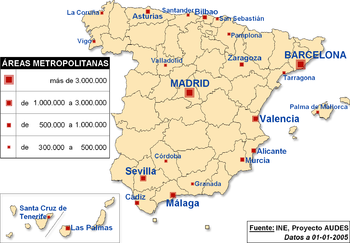
\includegraphics[width=.7\textwidth]{./image/cap3/Mapa_Espana1}
    %  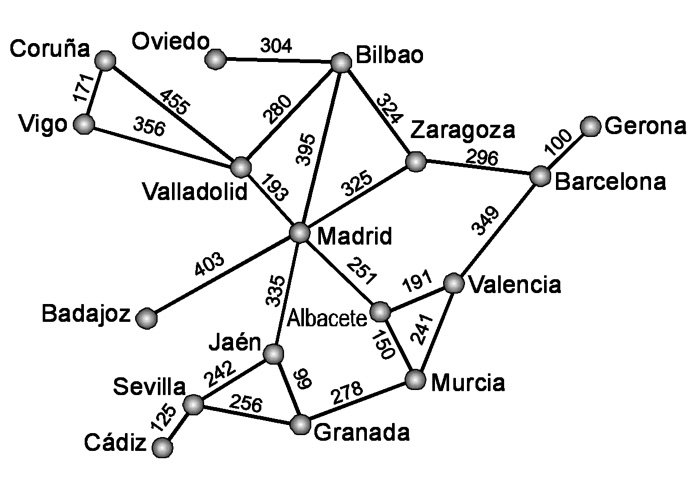
\includegraphics[width=.45\textwidth]{./image/cap3/Mapa_Espana2}
  \end{center}
  }
\end{frame}
\begin{frame}{Aplicación}
  \uncover<3>{
  \begin{center}
      %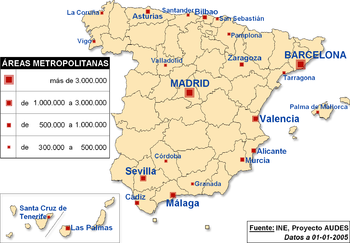
\includegraphics[width=.45\textwidth]{./image/cap3/Mapa_Espana1}
      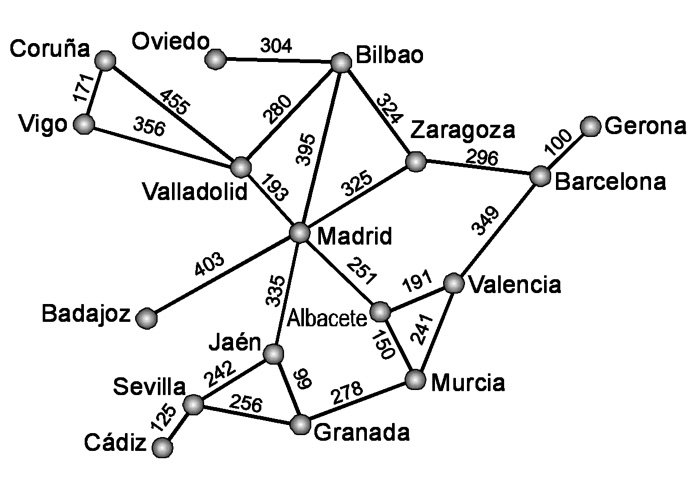
\includegraphics[width=.7\textwidth]{./image/cap3/Mapa_Espana2}
  \end{center}
  }
\end{frame}

\subsection{Representación}
\begin{frame}{Representación}
  \begin{itemize}
    \item La forma común de representar un grafo en memoria es mediante un arreglo bidimencional llamado Matriz de Adyacencia.
      \item \blue{Matríz de Adyacencia}: Es una matriz nxn donde n es la cantidad de nodos que forma al grafo y la posición i,j representa si hay o no arista entre los nodos siento este valor 1 o 0 si no es dirigido de un numero natural positivo si es un grafo dirigido.
  \end{itemize}
  \uncover<3>{
  \begin{center}
      %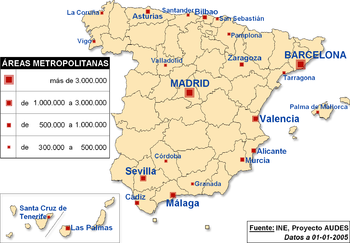
\includegraphics[width=.45\textwidth]{./image/cap3/Mapa_Espana1}
      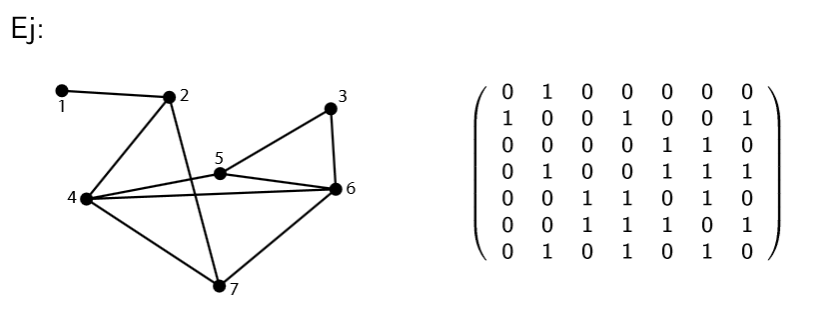
\includegraphics[width=.8\textwidth]{./image/cap3/Adyacencia}
  \end{center}
  }
\end{frame}

\begin{frame}{Representación - Matriz de Adyacencia}
  \begin{itemize}
    \item Esta es una de las representaciones más utilizadas. Si bien el ejemplo
es para un grafo no dirigido, también se puede utilizar la misma
estructura para grafos dirigidos y grafos con pesos.
\item Ventajas:
  \begin{itemize}
    \item Permite saber si existe o no arista entre dos nodos cualesquiera en O(1).
    \item Es muy fácil de implementar, matrizAdy[i][j] guarda toda la información sobre la arista.
  \end{itemize}
\item Desventajas:
  \begin{itemize}
    \item La complejidad espacial: se necesitan {n^{2}} \\ casillas para representar un grafo de n nodos.
  \end{itemize}
\end{itemize}

\end{frame}

\begin{frame}{Representación - Lista de Adyacencia}
  \begin{itemize}
    \item La lista de adyacencia es un vector de vectores de enteros, que en el
i-ésimo vector tiene el número j si hay una arista entre los nodos i y j.
\item También se le conoce como lista de vecinos ya que para cada nodo
se guarda la lista de nodos para los que existe una arista que los
conecta (o sea, los vecinos)

\end{itemize}
\uncover<3>{
\begin{center}
    %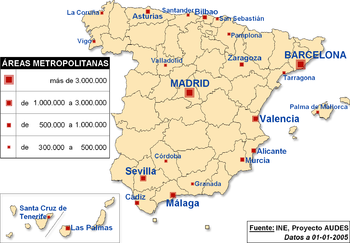
\includegraphics[width=.45\textwidth]{./image/cap3/Mapa_Espana1}
    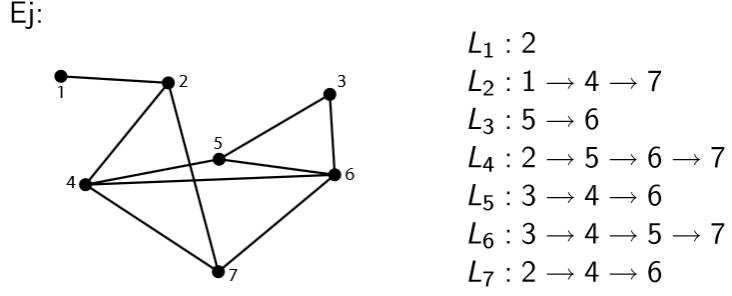
\includegraphics[width=.8\textwidth]{./image/cap3/Lista_Adyacencia}
\end{center}
}
\end{frame}

\begin{frame}{Representación - Lista de Adyacencia}
  \begin{itemize}
    \item Nuevamente, con la misma idea también se pueden modelar grafos
dirigidos y con pesos.
\item La complejidad espacial de esta representación será posiblemente
mucho menor. ¿Cuánta memoria necesitaremos para un grafo de n
nodos y m aristas? O(m+n)

\end{itemize}

\end{frame}

%-----------------------
\section{Recorrido}
\subsection{Camino más Corto}

\begin{frame}{Recorrido - Camino más Corto}
  \begin{itemize}
    \item Dado un grafo G con pesos en las aristas, el problema de camino
mínimo entre dos nodos u y v consiste en encontrar un camino entre
esos nodos cuyo peso sea menor o igual que el peso de cualquier otro
camino entre u y v

  \end{itemize}

\end{frame}

\subsection{Algoritmo de Dijkstra}
\begin{frame}{Recorrido - Algoritmo de Dijkstra}
  \begin{itemize}
    \item Este algoritmo fue creado por uno de los padres de la computación,
Edger W. Dijkstra, en 1956. Sirve para cualquier grafo con pesos
(dirigido o no) siempre y cuando sus pesos no sean negativos.

  \end{itemize}

\end{frame}

\begin{frame}{Recorrido - Algoritmo de Dijkstra}
  \begin{itemize}
    \item  El algoritmo calcula las distancias mínimas desde un nodo inicial
a todos los demás. Para hacerlo, en cada paso se toma el nodo
más cercano al inicial que aún no fue visitado (le diremos v). Este
nodo tiene calculada la menor distancia al nodo inicial (¿por
qué?).
\item Luego, recalculamos todas los caminos mínimos, teniendo en
cuenta a v como camino intermedio.
\item Así, en cada paso tendremos un subconjunto de nodos que ya
tienen calculada su mínima distancia y los demás tienen
calculada su mínima distancia si solo puedo usar los nodos del
conjunto como nodos intermedios.
\item Con cada iteración agregaremos un nodo más a nuestro conjunto,
hasta resolver el problema en su totalidad.
  \end{itemize}

\end{frame}

\subsection{Ejemplo}
\begin{frame}{Algoritmo de Dijkstra - Ejemplo}
\uncover<3>{
\begin{center}
    %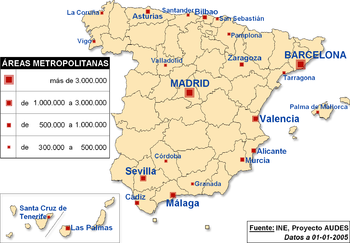
\includegraphics[width=.45\textwidth]{./image/cap3/Mapa_Espana1}
    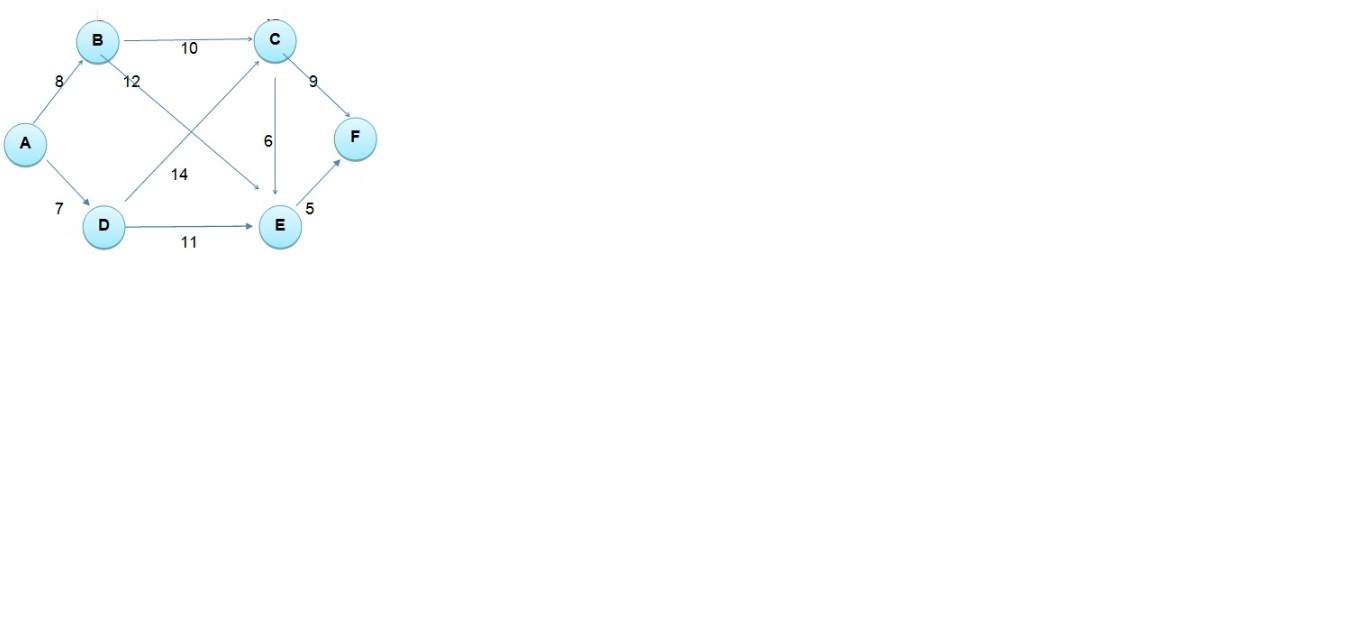
\includegraphics[width=2.5\textwidth]{./image/cap3/grafo01}
\end{center}
}
\end{frame}

\begin{frame}{Algoritmo de Dijkstra - Ejemplo}
\uncover<3>{
\begin{center}
    %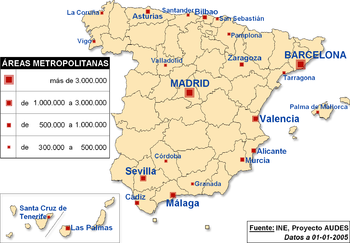
\includegraphics[width=.45\textwidth]{./image/cap3/Mapa_Espana1}
    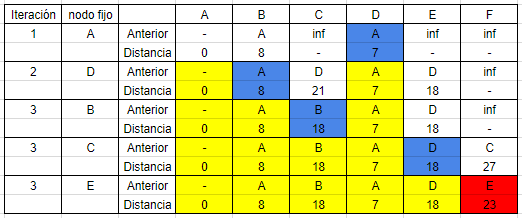
\includegraphics[width=.8\textwidth]{./image/cap3/grafo01_resp}
\end{center}
}

\begin{itemize}
  \item Respuesta:  A \rightarrow D \rightarrow E \rightarrow F
\end{itemize}
\end{frame}

\end{document}
